\Variant{23.11.2025}
\QQ{1}{$2!+4!+6!+\dots+2024!$ yiğindining oxirgi raqamini toping.
\Opts{$6$}{$8$}{$2$}{$0$}}
\QQ{2}{Hisoblang:
\[\left(4{,}(6)\cdot2\frac47-3\right)\cdot1{,}0(5)-\frac1{0{,}4}\]
\Opts{$5$}{$6$}{$7$}{$8$}}
\QQ{3}{Uçta poliz ekinlari tarvuz, qovun va karamlarning narxlari donasiga $50\,000$ söm, $10\,000$ söm va $1000$ sömdan narxlangan. Jami $500\,000$ sömlik xarid orqali $100$ ta mahsulot olingan bölsa, karamlar soni neçta?
\Opts{$58$}{$60$}{$52$}{$39$}}
\QQ{4}{Yoğliligi $36\%$ bölgan yangi soğilgan sutdan yoğ olib taşlangandan keyin yoğligi $4\%$ li sut qoladi. $18$ litr $4\%$ li sut oliş uçun qança yoği olinmagan sut kerak?
\Opts{$16$}{$36$}{$27$}{$9$}}
\QQ{5}{$n$ va $m$ sonlar uçun $4n+m=3$ bölsa, $3^m\cdot81^n$ ni hisoblang.
\Opts{$24$}{$27$}{$25$}{$21$}}
\QQ{6}{Hisoblang:
\[\sqrt{3{,}25+\sqrt3}+\sqrt{7-4\sqrt3}\]
\Opts{$5$}{$3$}{$\dfrac52$}{$\dfrac32$}}
\QQ{7}{Hisoblang:
\[\sqrt[3]{9+4\sqrt5}-\sqrt[3]{7-5\sqrt2}+\sqrt[3]{9-4\sqrt5}-\sqrt[3]{7+5\sqrt2}\]
\Opts{$3$}{$1$}{$-1$}{$2$}}
\QQ{8}{$\{a_n\}$ arifmetik progressiya hadlari $a_1=p$; $a_2=k$; $a_3=p^2$ ga teng. $\{b_n\}$ geometrik progressiya hadlari $b_1=p$, $b_2=p^2$, $b_3=k$ ga teng. Arifmetik progressiyaning dastlabki $10$ ta hadi yiğindisini toping. (Bunda $p\ne k$)
\Opts{$\dfrac{95}8$}{$\dfrac{85}7$}{$\dfrac{15}8$}{$\dfrac{97}8$}}
\QQ{9}{Kamayuvçi geometrik progressiya uçun $b_1^2+b_2^2+b_3^2=84$, $b_1+b_2+b_3=14$ bölsa, geometrik progressiyaning dastlabki oltita hadi yiğindisini toping.
\Opts{$13\dfrac14$}{$15\dfrac34$}{$14\dfrac14$}{$15\dfrac14$}}
\QQ{10}{Agar $b<c<0<a$ bölsa, ifodani soddalaştiring:
\[\frac{|b-a|}{ab}+\frac{|a-c|}{ac}+\frac{|b-c|}{bc}\]
\Opts{$\dfrac1{abc}$}{$\dfrac{2ab}3$}{$\dfrac{2a-2b}{ab}$}{$0$}}
\QQ{11}{Agar $a+b=x$, $ab=y$ bölsa, $ab^3+a^3b+a^2+b^2+5ab+2a^2b^2$ ni $x$ va $y$ orqali ifodalang.
\Opts{$xy^2+x^2+3y$}{$xy^2+y^2+2y$}{$yx^2+y^2+3y$}{$yx^2+x^2+3y$}}
\QQ{12}{Soddalaştiring:
\[\frac{\sin^22\alpha\cdot\tg^22\alpha}{1-\ctg^22\alpha}+\frac{\cos^22\alpha\cdot\ctg^22\alpha}{1-\tg^22\alpha}+2\]
\Opts{$\dfrac8{\sin^24\alpha}$}{$1$}{$\dfrac4{\sin^24\alpha}$}{$3+4\ctg^24\alpha$}}
\QQ{13}{$\sqrt5\sin x+\sin2x=0$ tenglamaning $\left[\dfrac\pi2;\,\dfrac{5\pi}2\right]$ oraliqdagi ildizlari yiğindisini toping.
\Opts{$3\pi$}{$2\pi$}{$\pi$}{$4\pi$}}
\QQ{14}{$\dfrac{3+a+2^{x+2}}{x+5}=0$ tenglama $a$ ning qanday qiymatlarida yeçimga ega böladi?
\Opts{$(-\infty;\,-3{,}125)\cup(-3{,}125;\,-3)$}{$(-\infty;\,-3)$}{$(-\infty;\,-2)$}{$(-\infty;\,-3{,}125)\cup(-3{,}125;\,-2)$}}
\QQ{15}{Tenglamani yeçing:
\[\frac{2\ln2-\ln5+\ln(2x+3)}{\ln x+\ln(x+3)}=1\]
\Opts{$2$}{$3$}{$1$}{$4$}}
\QQ{16}{Tenglama neçta haqiqiy ildizga ega?
\[\frac{(x+2)^2-9}{x+7}\cdot(x+7)=16\]
\Opts{$1$}{$2$}{$3$}{yeçimga ega emas}}
\QQ{17}{Tenglama neçta ildizga ega?
\[\left(x^2-x-1\right)^3+\left(x^2-3x-2\right)^3=\left(2x^2-4x-3\right)^3\]
\Opts{$6$ ta}{$2$ ta}{$4$ ta}{$3$ ta}}
\QQ{18}{Tengsizlikning butun yeçimlari yiğindisini toping.
\[\frac{x^2-5x+64}{x^2-10x+24}\le\frac{10}{4-x}\]
\Opts{$-5$}{$-4$}{$-3$}{$-1$}}
\QQ{19}{Tenglamaning haqiqiy ildizlari köpaytmasini toping.
\[\sqrt[6]{x^2+3x}+\sqrt[3]{x^2+3x}=6\]
\Opts{$-32$}{$32$}{$-64$}{$64$}}
\QQ{20}{$f(x)=ax^3+bx^2+cx+d$ funksiya grafigi tasvirlangan. Funksiya $(2;\,0)$ nuqtada $Ox$ öqiga urinadi. $Ox$ öqini $(-3;\,0)$ va $Oy$ öqini esa $(0;\,4)$ nuqtalarda kesib ötadi. $a+b+c+d$ ni toping.
\qfig{\begin{tikzpicture}[x=0.55cm,y=0.32cm,font=\small]
\draw[->] (-4.2,0)--(4.4,0) node[right] {$x$}; \draw[->] (0,-3.4)--(0,8) node[left] {$y$};
\draw[thick,domain=-3.3:3.25,samples=100] plot (\x,{(\x-2)*(\x-2)*(\x+3)/3});
\node[below left] at (-3,0) {$-3$}; \node[below] at (2,0) {$2$}; \node[right] at (0,4.3) {$4$};
\node[right] at (3.2,6.6) {$f(x)=ax^3+bx^2+cx+d$};
\end{tikzpicture}}
\Opts{$1$}{$\dfrac13$}{$\dfrac43$}{$2$}}
\QQ{21}{Hisoblang:
\[\int_2^4\frac3{(x-5)(x-1)}\,dx\]
\Opts{$\dfrac32\ln3$}{$\ln3$}{$-\dfrac32\ln3$}{$\dfrac52\ln2$}}
\QQ{22}{$f(x)=\cos\left(kx^n\right)\cdot\lg\sqrt[n]{x+\sqrt{1+x^2}}$ funksiya berilgan. Agar $f'(2023)=2024$ bölsa, $f'(-2023)+2024$ ni hisoblang.
\Opts{$0$}{$2024$}{$4096$}{$4048$}}
\QQ{23}{Rasmdagi aylanalar içki urinadi. Kiçik doiradan vatar ajratgan segment (rasmda $9$ bilan belgilangan) yuzi $9$ ga teng. Böyalgan soha yuzini toping.
\qfig{\begin{tikzpicture}[scale=0.95,font=\small]
\coordinate (T) at (2,0); \coordinate (P) at (-1.732,1); \coordinate (Q) at (-0.239,0.6);
\fill[qfill] (T) arc[start angle=0,end angle=150,radius=2] -- cycle;
\fill[white] (T) arc[start angle=0,end angle=150,radius=1.2] -- cycle;
\draw (0,0) circle (2); \draw (0.8,0) circle (1.2); \draw (P)--(T); \fill (0,0) circle (1.3pt);
\node[above] at ($(P)!0.5!(Q)$) {$2x$}; \node[below] at ($(Q)!0.5!(T)$) {$3x$}; \node at (0.85,0.75) {$9$};
\end{tikzpicture}}
\Opts{$16$}{$27$}{$18$}{$24$}}
\QQ{24}{$f(x)=\dfrac x4+\dfrac4x$ funksiyaning $[-6;\,-2]$ oraliqdagi eng katta qiymatini toping.
\Opts{$-\dfrac{13}6$}{$-\dfrac52$}{$-2$}{$-1$}}
\QQ{25}{Muntazam uçburçakning içidagi ixtiyoriy nuqtadan tomonlariga tuşirilgan perpendikulyarlar $3$, $4$ va $5$ ga teng bölsa, muntazam uçburçakning yuzini toping.
\Opts{$30\sqrt3$}{$24\sqrt3$}{$36\sqrt3$}{$48\sqrt3$}}
\QQ{26}{Rasmda uçta kvadrat tasvirlangan. Böyalgan soha yuzini toping.
\qfig{\begin{tikzpicture}[scale=0.42,font=\small]
\fill[qfill] (0,5.4)--(12,3)--(12,0)--cycle;
\draw (0,0) rectangle (5.4,5.4); \draw (5.4,0) rectangle (9,3.6); \draw (9,0) rectangle (12,3);
\draw (0,5.4)--(12,3); \draw (0,5.4)--(12,0);
\draw[dashed,<->,>=stealth] (0,-0.7)--(9,-0.7); \node[fill=white,inner sep=1pt] at (4.5,-0.7) {$9$}; \node at (10.5,-0.7) {$3$};
\end{tikzpicture}}
\Opts{$15$}{$24$}{$18$}{$21$}}
\QQ{27}{$ABC$ uçburçakda $A$ uçidan $BC$ tomonga $AD$ bissektrisa ötkazilgan. Bunda $BD:DC=1:2$, $AD=DC$ bölsa, $\alpha$ burçakni toping.
\qfig{\begin{tikzpicture}[scale=0.75,font=\small]
\coordinate (A) at (0,0); \coordinate (C) at (6,0); \coordinate (B) at (1.5,2.598); \coordinate (D) at (3,1.732);
\draw (A)--(B)--(C)--cycle; \draw (A)--(D);
\draw ($(B)!0.4cm!(A)$) arc (240:330:0.4cm); \node at ($(B)+(285:0.75)$) {$\alpha$};
\draw ($(A)!0.5cm!(C)$) arc (0:30:0.5cm); \draw ($(A)!0.6cm!(D)$) arc (30:60:0.6cm);
\node[below left] at (A) {$A$}; \node[above] at (B) {$B$}; \node[below right] at (C) {$C$}; \node[above right] at (D) {$D$};
\end{tikzpicture}}
\Opts{$60^\circ$}{$90^\circ$}{$45^\circ$}{$36^\circ$}}
\QQ{28}{Muntazam sakkizburçak tomonlarini davom ettirişdan hosil bölgan $\alpha$ va $\beta$ burçaklar yiğindisini toping.
\qfig{\begin{tikzpicture}[scale=0.9,font=\small]
\draw (22.5:1.5)--(67.5:1.5)--(112.5:1.5)--(157.5:1.5)--(202.5:1.5)--(247.5:1.5)--(292.5:1.5)--(337.5:1.5)--cycle;
\coordinate (P) at (3.346,1.386); \coordinate (Q) at (-1.96,0);
\draw (67.5:1.5)--(P)--(337.5:1.5); \draw (157.5:1.5)--(Q)--(202.5:1.5);
\draw ($(P)!0.45cm!(67.5:1.5)$) arc (180:225:0.45cm); \node at ($(P)+(202.5:0.75)$) {$\alpha$};
\draw ($(Q)!0.3cm!(157.5:1.5)$) arc (45:-45:0.3cm); \node at ($(Q)+(0:0.55)$) {$\beta$};
\end{tikzpicture}}
\Opts{$120^\circ$}{$150^\circ$}{$135^\circ$}{$130^\circ$}}
\QQ{29}{$\vec a$, $\vec b$, $\vec c$ birlik vektorlar va $\widehat{\vec a,\vec b}=\widehat{\vec b,\vec c}=\widehat{\vec a,\vec c}=60^\circ$ bölsa, $\vec a$ va $\vec b+\vec c$ vektorlar orasidagi burçak kosinusini hisoblang.
\Opts{$\dfrac2{\sqrt3}$}{$1$}{$\dfrac1{\sqrt3}$}{$\dfrac{\sqrt3}2$}}
\QQ{30}{Muntazam oltiburçakli piramidaning yon qirrasi asos tekisligi bilan $45^\circ$ burçak taşkil qiladi. Yon qirrasi $4\sqrt6$ ga teng bölsa, piramida hajmini toping.
\Opts{$128$}{$108$}{$144$}{$288$}}
\QQ{31}{$A$ va $B$ böş bölmagan töplamlar: $A=\{6$ ga karrali ikki xonali sonlar$\}$, $B=\{$yozuvida kamida bitta $6$ raqami bölgan ikki xonali sonlar$\}$. $A\cap B$ töplamning elementlari soni neçta?
\Opts{$4$}{$3$}{$5$}{$6$}}
\QQ{32}{Hasan va Husan markazdan $6$ ta teng sektorga bölingan aylana yöli böylab tasodifiy bir yönalişni tanlab, $1$ soat $5$ km/soat tezlikda yuradi. Şuning uçun ikkalasi ham markazdan $5$ km radiusli aylana böylab joylaşadi. $1$ soat harakatlangandan söng orasidagi masofa $6$ km dan kam bölmaslik ehtimolligi neçaga teng?
\qfig{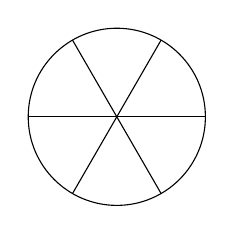
\begin{tikzpicture}[scale=0.75]
\draw (0,0) circle (1.5); \foreach \a in {0,60,...,300} \draw (0,0)--(\a:1.5);
\end{tikzpicture}}
\Opts{$\dfrac12$}{$\dfrac16$}{$\dfrac14$}{$\dfrac13$}}
\QQ{33}{\Moslash{Silindr va kesik konusdan iborat banka tasvirlangan bölib, bankaning hajmi $1000\pi$ cm$^3$, silindr balandligi kesik konus balandligidan $3$ marta katta bölib, kesik konus kiçik asosining diametri $8$ cm bölsa,
\par\centering\begin{tikzpicture}[x=0.13cm,y=0.13cm,font=\small]
\fill[qfill] (-6,0) arc[start angle=180,end angle=360,x radius=6,y radius=1.3] -- (6,12) arc[start angle=0,end angle=180,x radius=6,y radius=1.3] -- cycle;
\draw (6,12) arc[start angle=0,end angle=360,x radius=6,y radius=1.3];
\draw (-6,0) arc[start angle=180,end angle=360,x radius=6,y radius=1.3]; \draw[dashed] (6,0) arc[start angle=0,end angle=180,x radius=6,y radius=1.3];
\draw (-6,0)--(-6,22.5); \draw (6,0)--(6,22.5); \draw (0,22.5) ellipse (6 and 1.3);
\draw (-6,22.5)--(-4,30); \draw (6,22.5)--(4,30); \draw (0,30) ellipse (4 and 0.9);
\draw[dashed] (-12,0)--(-6,0); \draw[dashed] (-12,30)--(-4,30); \draw[<->,>=stealth] (-11,0)--(-11,30); \node[left] at (-11,15) {$30$};
\draw[dashed] (4,30)--(12,30); \draw[dashed] (6,22.5)--(12,22.5); \draw[<->,>=stealth] (11,22.5)--(11,30); \node[right] at (11,26.25) {$h_1$};
\draw[dashed] (6,12)--(12,12); \draw[dashed] (6,0)--(12,0); \draw[<->,>=stealth] (11,0)--(11,12); \node[right] at (11,6) {$h_2$};
\draw[<->,>=stealth] (-4,33)--(4,33); \node[fill=white,inner sep=1pt] at (0,33) {$8$}; \draw[dashed] (-4,30)--(-4,33.5); \draw[dashed] (4,30)--(4,33.5);
\end{tikzpicture}}{A) $4{,}5$\par B) $7{,}5$\par C) $8$\par D) $6$\par E) $14$\par F) $12$}{Kesik konus balandligini ($h_1$) toping.}{Silindr asosining radiusini toping.}{Banka içidagi sut (rasmga qarang) hajmi $432\pi$ cm$^3$ bölsa, sut mavjud bölgan balandlikni ($h_2$) toping.}}
\QQ{36}{Tenglama berilgan:
\[x^4+kx^3+x^2+4kx+16=0\]
\AB{Tenglama $k=1$ bölganda neçta haqiqiy ildizga ega böladi?}{Tenglama yagona ildizga ega böladigan $k$ ning qiymatlari neçta?}}
\QQ{37}{Tenglama berilgan:
\[\tg3x+\ctg\frac{3x}2=\cos^2\frac{3x}2\]
\AB{Tenglama $[0;\,\pi]$ oraliqda neçta yeçimga ega?}{Tenglamaning eng katta manfiy va eng kiçik musbat ildizlari yiğindisini toping.}}
\QQ{38}{$f(x)=-|x-a|+b$ va $g(x)=|x-c|+d$ funksiya grafiklari berilgan. $f(x)$ va $g(x)$ funksiya grafiklari $A(2;\,5)$ va $B(8;\,3)$ nuqtalarda kesişadi. Rasmdagi maʼlumotlar asosida
\qfig{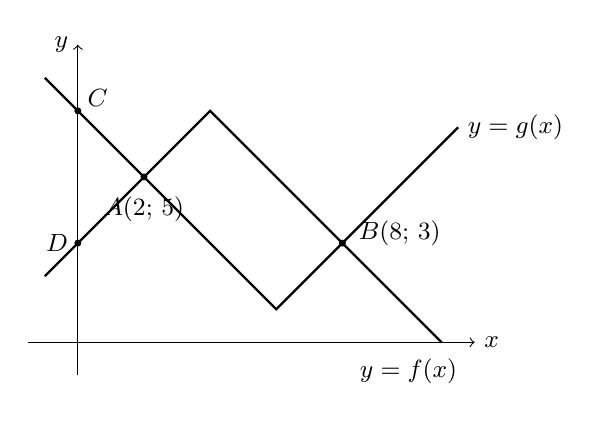
\begin{tikzpicture}[scale=0.42,font=\small]
\draw[->] (-1.5,0)--(12,0) node[right] {$x$}; \draw[->] (0,-1)--(0,9) node[left] {$y$};
\draw[thick] (-1,2)--(4,7)--(11,0); \draw[thick] (-1,8)--(6,1)--(11.5,6.5);
\fill (2,5) circle (3pt); \fill (8,3) circle (3pt); \fill (0,7) circle (3pt); \fill (0,3) circle (3pt);
\node[below] at (2,4.7) {$A(2;\,5)$}; \node[right] at (8.2,3.3) {$B(8;\,3)$}; \node[right] at (0,7.4) {$C$}; \node[left] at (0,3) {$D$};
\node[right] at (11.5,6.5) {$y=g(x)$}; \node[below] at (10,-0.2) {$y=f(x)$};
\end{tikzpicture}}
\AB{$\dfrac{b+d}{c-a}$ ni toping.}{$C$ va $D$ nuqtalar orasidagi masofani toping.}}
\QQ{39}{Rasmda $\varphi(x)$ funksiya grafigi tasvirlangan bölib, rasmdagi maʼlumotlar asosida
\qfig{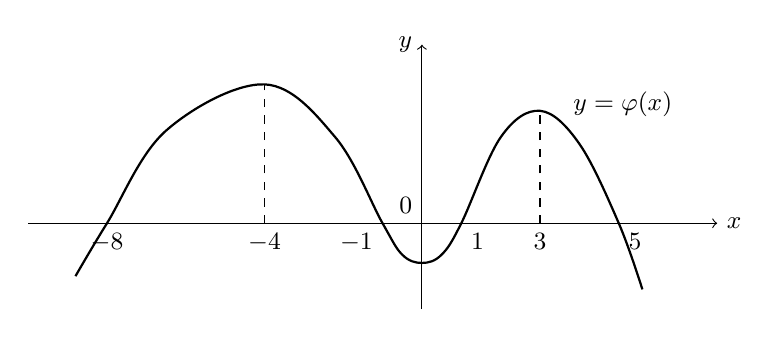
\begin{tikzpicture}[x=0.5cm,y=0.42cm,font=\small]
\draw[->] (-10,0)--(7.5,0) node[right] {$x$}; \draw[->] (0,-2.6)--(0,5.4) node[left] {$y$};
\draw[thick] plot[smooth,tension=0.6] coordinates {(-8.8,-1.6) (-8,0) (-6.5,2.8) (-4,4.2) (-2.2,2.6) (-1,0) (-0.5,-0.95) (0,-1.2) (0.5,-0.95) (1,0) (2,2.6) (3,3.4) (4,2.4) (5,0) (5.6,-2)};
\draw[dashed] (-4,0)--(-4,4.2); \draw[dashed] (3,0)--(3,3.4);
\node[below] at (-8,0) {$-8$}; \node[below] at (-4,0) {$-4$}; \node[below left] at (-1,0) {$-1$}; \node[below right] at (1,0) {$1$}; \node[below] at (3,0) {$3$}; \node[below right] at (5,0) {$5$}; \node[above left] at (0,0) {$0$};
\node[right] at (3.6,3.6) {$y=\varphi(x)$};
\end{tikzpicture}}
\AB{$\dfrac{x\varphi(x)}{\varphi'(x)}<0$ tengsizlik $(-8;\,5)$ oraliqda neçta butun yeçimga ega böladi?}{$\begin{cases}\varphi(x)>0\\ \varphi'(x)>0\end{cases}$ tengsizliklar sistemasi $(-8;\,5)$ oraliqda neçta butun yeçimga ega?}}
\QQ{40}{Rasmda $f(x)$ va $g(x)$ funksiya grafiklari tasvirlangan. Berilgan maʼlumotlar asosida
\qfig{\begin{tikzpicture}[x=1.1cm,y=0.5cm,font=\small]
\fill[qfill] plot[domain=0:2,samples=60] (\x,{\x*(\x-2)*(\x-2)}) -- plot[domain=2:0,samples=60] (\x,{\x*\x*(\x-2)}) -- cycle;
\draw[->] (-1,0)--(3.6,0) node[right] {$x$}; \draw[->] (0,-2.2)--(0,6) node[left] {$y$};
\draw[thick,domain=-0.55:3.15,samples=100] plot (\x,{\x*(\x-2)*(\x-2)});
\draw[thick,domain=-0.75:2.75,samples=100] plot (\x,{\x*\x*(\x-2)});
\node[below left] at (0,0) {$0$}; \node[below right] at (2,0) {$2$};
\node[right] at (3.1,4.2) {$f(x)=x^3+ax^2+bx+c$}; \node[right] at (0.2,-1.8) {$g(x)=x^3+px^2+qx+d$};
\end{tikzpicture}}
\AB{$\dfrac{a+b+c}{p+q+d}$ ni toping.}{Böyalgan soha yuzini toping.}}
\QQ{41}{$ABC$ uçburçakda $B$ uçidan $BP$ — bissektrisa, $BH$ — balandlik, $BM$ — mediana ötkazilgan. $L$ — içki çizilgan aylananing $AC$ ga uriniş nuqtasi (rasmga qarang).
\qfig{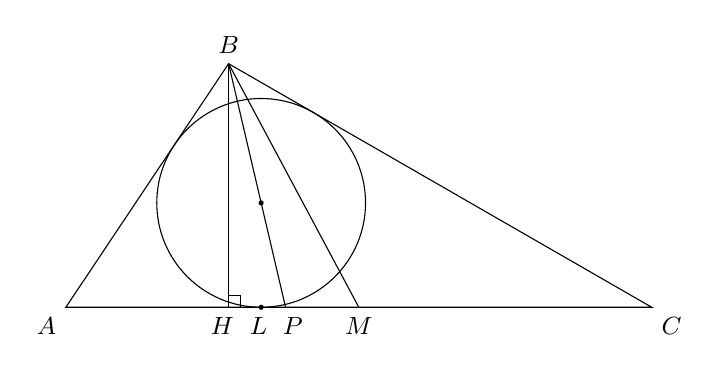
\begin{tikzpicture}[scale=0.62,font=\small]
\coordinate (A) at (0,0); \coordinate (C) at (12,0); \coordinate (B) at (3.333,4.989); \coordinate (H) at (3.333,0); \coordinate (L) at (4,0); \coordinate (P) at (4.5,0); \coordinate (M) at (6,0); \coordinate (I) at (4,2.138);
\draw (A)--(B)--(C)--cycle; \draw (B)--(H); \draw (B)--(P); \draw (B)--(M); \draw (I) circle (2.138); \fill (I) circle (1.5pt); \fill (L) circle (1.5pt);
\draw (3.333,0.25)--(3.583,0.25)--(3.583,0);
\node[below left] at (A) {$A$}; \node[above] at (B) {$B$}; \node[below right] at (C) {$C$};
\node[below] at (3.2,0) {$H$}; \node[below] at (3.95,0) {$L$}; \node[below] at (4.65,0) {$P$}; \node[below] at (M) {$M$};
\end{tikzpicture}}
\AB{$AB=4$, $BC=6$ bölsa, $LM$ ni toping.}{$AB=6$, $BC=10$, $AC=12$ bölsa, $HL$ ni toping.}}
\QQ{42}{$ABCD$ kvadrat berilgan.
\qfig{\begin{tikzpicture}[scale=1.25,font=\small]
\coordinate (D) at (0,0); \coordinate (C) at (2.798,0); \coordinate (B) at (2.798,2.798); \coordinate (A) at (0,2.798); \coordinate (E) at (0.863,0.505);
\fill[qfill] (D)--(E)--(B)--cycle;
\draw (A)--(B)--(C)--(D)--cycle; \draw (D)--(E)--(B); \draw (E)--(C);
\draw ($(E)!0.25cm!(D)$) arc[start angle=210.3,end angle=345.4,radius=0.25cm]; \node at ($(E)+(275:0.42)$) {\scriptsize$\alpha$};
\node[above left] at (A) {$A$}; \node[above right] at (B) {$B$}; \node[below right] at (C) {$C$}; \node[below left] at (D) {$D$}; \node[above] at (0.95,0.55) {$E$};
\node[above left] at (0.43,0.25) {$1$}; \node[above] at (1.83,0.25) {$2$}; \node[right] at (1.85,1.7) {$3$};
\end{tikzpicture}}
\AB{$\angle DEC$ ni toping.}{Böyalgan soha yuzini toping.}}
\QQ{43}{$ABCDE$ beşburçakka taşqi aylana çizilgan (rasmga qarang). $AB=BC=CD=DE=4$, $\angle ADB=30^\circ$, $F$ nuqta $AD$ va $BE$ diagonallar kesişiş nuqtasi bölsa,
\qfig{\begin{tikzpicture}[scale=0.42,font=\small]
\coordinate (C) at (90:4); \coordinate (B) at (150:4); \coordinate (D) at (30:4); \coordinate (A) at (210:4); \coordinate (E) at (330:4); \coordinate (F) at (0,0);
\draw (0,0) circle (4); \draw (A)--(B)--(C)--(D)--(E)--cycle; \draw (B)--(D); \draw (A)--(D); \draw (B)--(E);
\draw ($(D)!0.6cm!(B)$) arc (180:210:0.6cm); \node at ($(D)+(195:1.4)$) {\scriptsize$30^\circ$};
\node[left] at (A) {$A$}; \node[left] at (B) {$B$}; \node[above] at (C) {$C$}; \node[right] at (D) {$D$}; \node[right] at (E) {$E$}; \node[below] at (F) {$F$};
\node[above left] at ($(B)!0.5!(C)$) {$4$}; \node[above right] at ($(C)!0.5!(D)$) {$4$}; \node[left] at ($(A)!0.5!(B)$) {$4$}; \node[right] at ($(D)!0.5!(E)$) {$4$};
\end{tikzpicture}}
\AB{$BCDF$ törtburçak yuzini toping.}{$AEF$ uçburçak yuzini toping.}}
\QQ{44}{Qalam konus va silindrsimon şakllardan iborat bölib, qalamning uzunligi $160$ mm bölib, $x$ ning uzunligi $y$ ning uzunligidan $130$ mm ga uzun va diametri $10$ mm bölsa,
\qfig{\begin{tikzpicture}[x=0.06cm,y=0.06cm,font=\small]
\fill[qfill] (0,-5)--(145,-5)--(160,0)--(145,5)--(0,5)--cycle;
\draw (0,-5)--(145,-5)--(160,0)--(145,5)--(0,5); \draw (0,0) ellipse (1.6 and 5); \draw (145,-5)--(145,5);
\draw[|<->|,>=stealth] (0,9)--(145,9); \node[fill=white,inner sep=1pt] at (72,9) {$x$};
\draw[|<->|,>=stealth] (145,9)--(160,9); \node[above] at (152.5,10) {$y$};
\draw[|<->|,>=stealth] (0,-9)--(160,-9); \node[fill=white,inner sep=1pt] at (80,-9) {$160$ mm};
\node[left] at (-12,8) {$10$ mm}; \draw[->,>=stealth] (-12,8) to[out=0,in=110] (0,2);
\end{tikzpicture}}
\AB{Qalamning konussimon uçi hajmini (mm$^3$) toping.}{Qalamning bir qismi bölgan silindr hajmini (mm$^3$) toping.}}
\QQ{45}{Uyning tom qismi asosi töğri burçakli uçburçak bölgan töğri prizmadan, tomning qiyalangan ikki yon yoği tunukadan iborat. Uyning pastki bölagi yaʼni parallelepiped şaklidagi qismi yoğoç bilan qoplangan. Parallelepipedning $2$ ta yon yoği kvadratdan va töğri törtburçakdan iborat (rasmga qarang).
\qfig{\begin{tikzpicture}[scale=0.3,font=\small]
\coordinate (F0) at (0,0); \coordinate (F1) at (12,0); \coordinate (F2) at (12,12); \coordinate (F3) at (0,12);
\coordinate (K0) at (-4.5,2.3); \coordinate (K3) at (-4.5,14.3); \coordinate (Hf) at (-2.88,13.47); \coordinate (R) at (-2.88,15.87); \coordinate (R2) at (9.12,15.87);
\fill[qfill] (F3)--(R)--(R2)--(F2)--cycle; \fill[qfill!45] (K3)--(R)--(F3)--cycle;
\draw (F0)--(F1)--(F2)--(F3)--cycle; \draw (F0)--(K0)--(K3)--(F3); \draw (K3)--(R)--(F3); \draw (R)--(R2)--(F2);
\draw[dashed] (R)--(Hf);
\node[below] at (6,12) {$12$}; \node[right] at (12,6) {$12$};
\node[below] at (-1.3,12.7) {\scriptsize$3{,}2$}; \node[left] at (-7,10.5) {\scriptsize$1{,}8$}; \draw[->,>=stealth] (-7,10.5) to[out=0,in=-90] (-3.69,13.8);
\end{tikzpicture}}
\AB{Tunukadan iborat qismi (ikkita yon yoq)ning yuzasini toping.}{Tunuka qismiga $1$ m$^2$ iga $180\,000$ sömdan, yoğoç bilan qoplangan qismiga $1$ m$^2$ iga $80\,000$ sömdan pul sarflansa, uyning tomini yaʼni $2$ ta qismiga tunuka va $4$ ta yon yoğini yoğoç bilan qoplaş uçun qança pul (söm) sarflanadi?}}
\Javoblar{A C B C B C B A B C D C A A C A A A C C C D A C D C B C C D A A B D F}{%
\OK{36}{$0$}{$2$}\OK{37}{$2$}{$0$}\OK{38}{$4$}{$4$}\OK{39}{$4$}{$4$}\OK{40}{$0$}{$\dfrac83$}%
\OK{41}{$1$}{$\dfrac23$}\OK{42}{$135^\circ$}{$\dfrac12$}\OK{43}{$8\sqrt3$}{$4\sqrt3$}\OK{44}{$125\pi$}{$3625\pi$}\OK{45}{$84$}{$47\,760\,000$}}
